\subsection{\href{http://www.gruponoto.com}{Noto Group S.A.}}
   \hypertarget{subsec:noto}
   Para la empresa Noto Group S.A se desarrollan y se fabrican actualmente
   equipos electrónicos para electromedicina estética entre los que se destacan: \\
      \cvlistitem{Radiofrecuencia tripolar.}
      \cvlistitem{Electroporador.}
      \cvlistitem{Microdermoabrasión.}
      \cvlistitem{Cavitador.}
      \cvlistitem{Luminoterapia.}
      \cvlistitem{Electroestimulador portátil.}
      \cvlistitem{Fuentes de alimentación categoría medica.}

      En la figuras \ref{fig:noto1}, \ref{fig:noto2} y \ref{fig:noto3} se muestran algunos de los equipos desarrollados y fabricados:
   \begin{figure}
      \begin{center}
         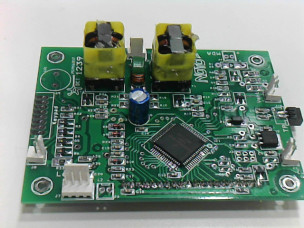
\includegraphics[width=0.24\textwidth]{noto5.jpg}
         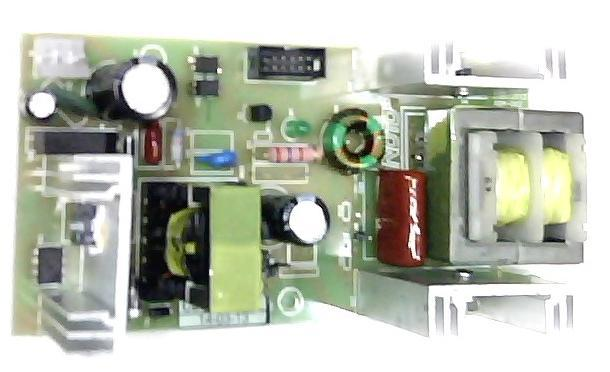
\includegraphics[width=0.24\textwidth]{noto6.jpg}
         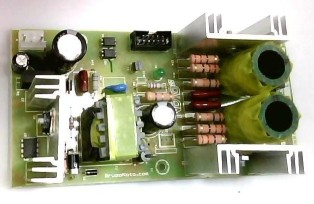
\includegraphics[width=0.24\textwidth]{noto7.jpg}
         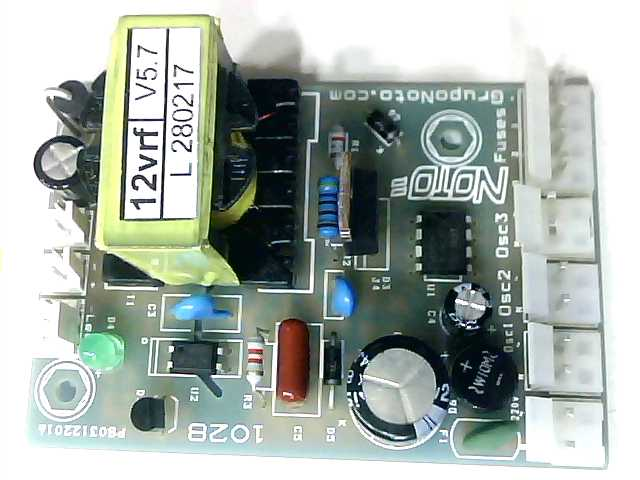
\includegraphics[width=0.24\textwidth]{noto8.jpg}
      \end{center}
      \caption{Equipos de potencia, fuentes, osciladores, mezclando tecnologias TH y SMD}
      \label{fig:noto1}
   \end{figure}
   \begin{figure}
      \begin{center}
         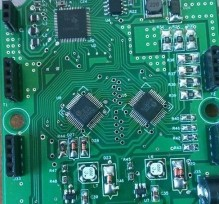
\includegraphics[width=0.24\textwidth]{noto9.jpg}
         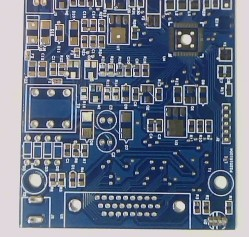
\includegraphics[width=0.24\textwidth]{noto10.jpg}
         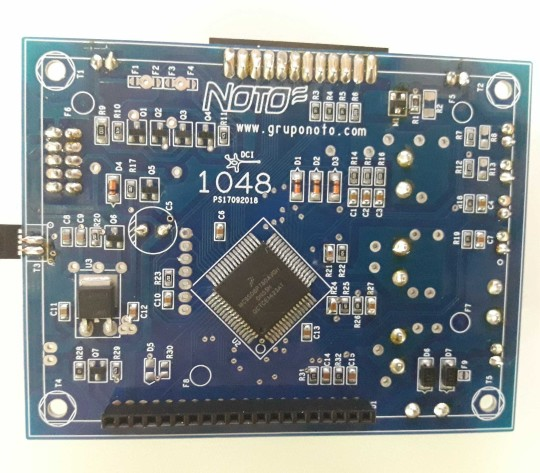
\includegraphics[width=0.24\textwidth]{noto11.jpg}
         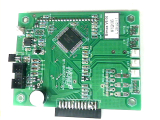
\includegraphics[width=0.24\textwidth]{noto12.jpg}
      \end{center}
      \caption{Placas de control para los diversos equipos, controladores de LCD, manejo de PWM, comunicaciones, generadores de señales, tecnología TH y SMD 1206, 0805 y 0603.}
      \label{fig:noto2}
   \end{figure}
   \begin{figure}
      \begin{center}
         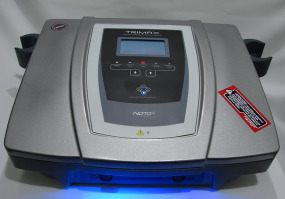
\includegraphics[width=0.24\textwidth]{noto1.jpg}
         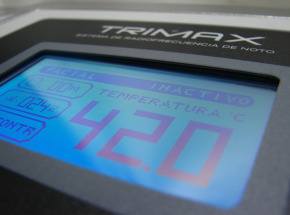
\includegraphics[width=0.24\textwidth]{noto2.jpg}
         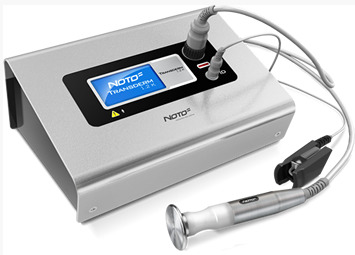
\includegraphics[width=0.24\textwidth]{noto3.jpg}
         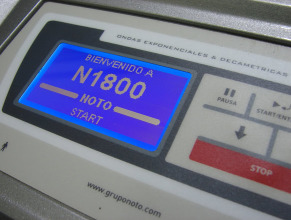
\includegraphics[width=0.24\textwidth]{noto4.jpg}
      \end{center}
      \caption{Equipos ensamblados y comercializados por la empresa Noto Group}
      \label{fig:noto3}
   \end{figure}
